\documentclass[xcolor=dvipsnames,aspectratio=169,t]{beamer}
  % t means frames are vertically centered to the top
\usepackage{slides-header}
\title{Markov Chains}

\renewcommand{\p}{\ensuremath{\mathbf{p}}}

\begin{document}
\maketitle

\begin{frame}{Monopoly}
  \begin{columns}[T]
  \column{.51\textwidth}
  \bigskip

  Monopoly is a board game where tokens are moved around the board. Players start on ``Go''.%
  \bigskip
  
  On each turn, a player rolls two dice, and then advances their token by the number of spaces equal to the sum of the rolled dice.
  \bigskip
  
  What is the most landed on spot in Monopoly?
  
  \column{.47\textwidth}
  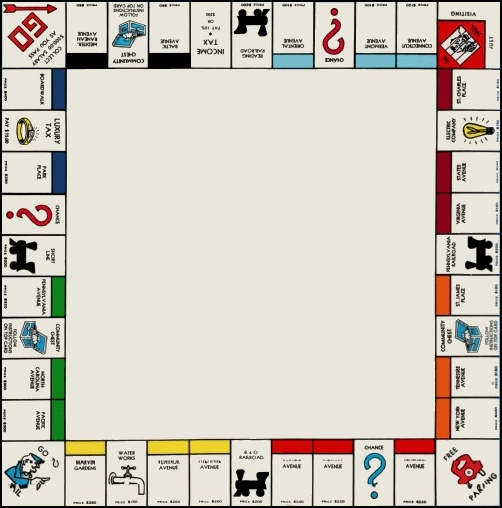
\includegraphics[scale=0.525]{images/Monopoly-board.png}
  \end{columns}
\end{frame}


\begin{frame}{Simplified Monopoly}
  \begin{columns}[T]
  \column{.6\textwidth}
  \medskip
  
  We'll use a board with 12 spaces (4 on each side),
  and roll 1 \blue{4-sided die} (numbered 1,2,3,4) on each turn.
  \medskip
  
  Players start on space 0 (``Go'').
  \medskip

  If a player lands on space 9 (``Go to Jail''), then when they leave on their next turn, they go to spaces $4,\ldots,7$.
  \bigskip
  
  Where will a player be after their \alert{first turn}?
  \medskip
  
  \onslide*<2->{
  A \alert{state} is the current space a player's token is on.
  \smallskip
  
  A \alert{state vector} gives a probability distribution on the states.
  \[ \x_1 = \begin{bmatrix} 0 & .25 & .25 & .25 & .25 & 0 & 0 & \ldots & 0 \end{bmatrix} \]
  }
  
  \column{.4\textwidth}
  \bigskip
  
  \hspace*{1em}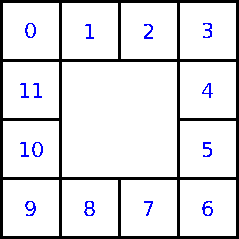
\includegraphics[scale=1.25]{images/Simplified_Monopoly_Board.pdf}
  \end{columns}

\end{frame}


\begin{frame}{Simplified Monopoly, continued}
  \medskip

  Where will a player be after their \alert{second turn} if they start at space $0$?
  \medskip
  
  \pause
  Let $\p_i$ give the probability distribution on states after one turn if the player \alert{starts} on space $i$.
  
  \[
    \text{Then }
    \x_2 = x_{11} \p_1 + x_{12} \p_2 + \ldots + x_{1n} \p_n
    \onslide<3->{= P \x_1, 
    \text{ where $P=\begin{bmatrix}\p_1 & \p_2 & \ldots & \p_n \end{bmatrix}$.}}
  \]
  \vspace*{-.75em}
  
  \pause
  $P=[p_{ij}]$ is the \blue{transition matrix}, where $p_{ij}$ is the prob of transitioning from \alert{state $j$} to \alert{state $i$}.
  \bigskip
  
  \pause
  \emph{Switch to Jupyter Notebook for calculations.}
  \bigskip

\end{frame}


\begin{frame}{Markov Chains}
  
  \begin{definition}
    A \alert{Markov chain} is a mathematical model used to describe a random process where:
    \begin{itemize}
      \item At each discrete time $k\ge 0$, the system is in one of $n$ \blue{states}.
      \item There are probabilities that describe how likely it is the system transitions from one state to another.
      These probabilities depend \alert{only} on the \alert{current state}.
    \end{itemize}
    {\small (\emph{We will only discuss discrete-time Markov chains with a finite number of states.})}
  \end{definition}
  \smallskip
  
  \pause
  Since a Markov chain describes a random process, we let the \blue{state vector} $\x_k$ be the probability distribution over which state the system is in at time $k$.
  \medskip
  
  The \blue{transition matrix} $P=[p_{ij}]$ has $p_{ij}=$ probability of transitioning from \alert{state $j$} to \alert{state $i$}.
  \medskip
  
  \pause
  The sequence $\x_0,\x_1,\x_2,\ldots$ of state vectors satisfies $\x_{k+1}=P\x_k$ for $k\ge 0$, 
  \pause
  and hence 
  \[ \x_{k+1} = P\x_k = P (P \x_{k-1}) = P^2 \x_{k-1} = \cdots = P^{k+1} \x_0. \]
\end{frame}




\begin{frame}{A Simple Weather Model}
  \smallskip
  
  \bi
  \ii Imagine that there are two possible states for weather: no rain (sunny) or rain.
  \ii You can always directly observe the current weather state.
  \ii The current weather has some bearing on what the next day’s weather will be.
  \ei
  \medskip

  \begin{columns}[T]

  \column{0.475\tw}

  \textbf{You want to be able to predict what the weather will be like tomorrow.}
  \pause

  \begin{center}
  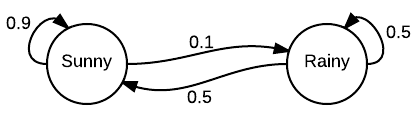
\includegraphics[width=0.9\tw]{images/fig-weather.png}
  \end{center}

  We can build a model to predict tomorrow's weather based on the weather \alert{today}.

  \column{0.5\tw}

  \[ P = \begin{bmatrix} 0.9 & 0.5 \\ 0.1 & 0.5 \end{bmatrix} \]

  \bi
  \ii We organize the probabilities of transitioning from one state to another in a \alert{transition matrix}.
  \ii $p_{ij}$ is the probability of transitioning from \alert{state $j$} to \alert{state $i$}.
  \ii This will be a \alert{stochastic matrix}. The entries in each column vector add up to 1.
  \ei

  \end{columns}
\end{frame}


\begin{frame}{A Simple Weather Model}
  \bigskip

  \begin{columns}[T]
  \column{0.5\tw}

  \begin{center}
  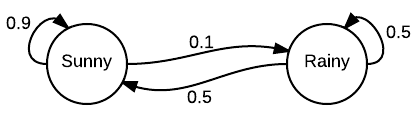
\includegraphics[width=0.9\tw]{images/fig-weather.png}
  \end{center}

  Today the weather is \alert{sunny}.
  \medskip
  
  state 1 = \alert{sunny}, \ state 2 = \blue{rainy}

  \[ \x_0 = \begin{bmatrix} 1 \\ 0 \end{bmatrix} \]
  \vspace*{-.5em}

  What is the probability that it \blue{rains} three days from now?

  \column{0.5\tw}

  \pause
  \begin{align*}
  \x_3 &= P \alert{\x_2} = P \alert{P \x_1} = P \alert{P P \x_0} = P^3 \x_0 \\
  &= \begin{bmatrix} 0.9 & 0.5 \\ 0.1 & 0.5 \end{bmatrix}^3 \begin{bmatrix} 1 \\ 0 \end{bmatrix} \\
  &= \begin{bmatrix} 0.844 \\ 0.156 \end{bmatrix}
  \end{align*}
  
  So the probability it \blue{rains} in three days, given that today is \alert{sunny}, is $0.156$.
  
  \end{columns}
\end{frame}

\begin{frame}{Modeling Election Outcomes}

\begin{columns}[T]

\column{0.5\tw}

Consider the following model:

\begin{center}
\includegraphics[width=0.7\tw]{images/fig-voting.png}
\end{center}

\vspace{-0.7in}

\[ \mbox{With initial state vector } \quad \x_0 = \begin{bmatrix} 0.50 \\ 0.45 \\ 0.05 \end{bmatrix} \]


\column{0.5\tw}

\bb
\ii What is the predicted outcome in the next election cycle? 
\ii What is the predicted outcome in two election cycles?
\ee


\[  \begin{bmatrix}
0.7 & 0.1 & 0.3 \\
0.2 & 0.8 & 0.3 \\
0.1 & 0.1 & 0.4 \end{bmatrix} \begin{bmatrix} 0.5 \\ 0.45 \\ 0.05 \end{bmatrix}  = 
\begin{bmatrix} 0.41 \\ 0.475 \\ 0.115 \end{bmatrix} \]

\[  \begin{bmatrix}
0.7 & 0.1 & 0.3 \\
0.2 & 0.8 & 0.3 \\
0.1 & 0.1 & 0.4 \end{bmatrix} \begin{bmatrix} 0.41 \\ 0.475 \\ 0.115 \end{bmatrix} = 
\begin{bmatrix} 0.369 \\ 0.4965 \\ 0.1345 \end{bmatrix} \]

\end{columns}

\end{frame}

\begin{frame}{Long Term Predictions}
  \smallskip

  Often we are interested in making predictions far out in time.
  \bi
  \ii Based on migration patterns, what is the long term prediction for the population of a certain species?
  \ii Based on current infection rates, what is the long term prediction for the total number of infected people?
  \ei

  \[ \x_k = P^k \x_0 \quad \mbox{for large } k \]
  \vspace*{-.2em}

  \pause
  Under some reasonable assumptions,
  the limiting distribution $\x_\infty$ will satisfy
  \[ \x_\infty = P \x_\infty. \]

  \pause
  The limiting distribution is an \alert{eigenvector} of $P$ corresponding to the \alert{eigenvalue 1!}
  \medskip

  \pause
  The limiting distribution does \alert{not} depend on the initial state vector $\x_0$.
\end{frame}


\begin{frame}{Long Term Predictions}

\bb
\ii What is the predicted outcome in the next election cycle? 
\ii What is the predicted outcome in two election cycles?
\ii What is the predicted political demographics in the long-run?
\ee

\pause
{\small
\[ \x_1 =  \begin{bmatrix}
0.7 & 0.1 & 0.3 \\
0.2 & 0.8 & 0.3 \\
0.1 & 0.1 & 0.4 \end{bmatrix} \begin{bmatrix} 0.5 \\ 0.45 \\ 0.05 \end{bmatrix}  = 
\begin{bmatrix} 0.41 \\ 0.475 \\ 0.115 \end{bmatrix} \quad
 \x_2 =   \begin{bmatrix}
0.7 & 0.1 & 0.3 \\
0.2 & 0.8 & 0.3 \\
0.1 & 0.1 & 0.4 \end{bmatrix} \begin{bmatrix} 0.41 \\ 0.475 \\ 0.115 \end{bmatrix} = 
\begin{bmatrix} 0.369 \\ 0.4965 \\ 0.1345 \end{bmatrix} \] }

\vspace{-0.1in}

\pause
{\small 
\[ \x_{10} =  \begin{bmatrix}
0.7 & 0.1 & 0.3 \\
0.2 & 0.8 & 0.3 \\
0.1 & 0.1 & 0.4 \end{bmatrix}^{10} \begin{bmatrix} 0.5 \\ 0.45 \\ 0.05 \end{bmatrix} = 
\begin{bmatrix} 0.3221 \\ 0.5350 \\ 0.1429  \end{bmatrix} \quad
 \x_{20} =  \begin{bmatrix}
0.7 & 0.1 & 0.3 \\
0.2 & 0.8 & 0.3 \\
0.1 & 0.1 & 0.4 \end{bmatrix}^{20} \begin{bmatrix} 0.5 \\ 0.45 \\ 0.05 \end{bmatrix} = 
\begin{bmatrix} 0.3214 \\ 0.5357  \\ 0.1429 \end{bmatrix} \] }

\vspace{-0.1in}

\pause
{\small
\[ \x_{30} =  \begin{bmatrix}
0.7 & 0.1 & 0.3 \\
0.2 & 0.8 & 0.3 \\
0.1 & 0.1 & 0.4 \end{bmatrix}^{30} \begin{bmatrix} 0.5 \\ 0.45 \\ 0.05 \end{bmatrix} = 
\alert{\begin{bmatrix} 0.3214 \\ 0.5357 \\  0.1429\end{bmatrix}} \] }
\end{frame}


\begin{frame}{Steady State Vectors}
  \bbox
  If $P$ is a stochastic matrix, then a \alert{steady state vector} (or \alert{equilibrium vector}) for $P$ is a \colorb{probability vector $\mathbf{q}$} (nonnegative entries that sum to $1$) such that 
  \[ P \mathbf{q} = \mathbf{q}. \]

  \bi
  \ii Note that $\mathbf{q}$ is an eigenvector of $P$ corresponding to $\lambda = 1$.
  \ii Thus if probability vector $\mathbf{q}$ is an eigenvector of $\lambda =1$, it is a steady state vector.
  \ei
  \ebox

  \pause
  \begin{columns}[T]
  \column{.6\textwidth}
  Elections example

  \[ \begin{bmatrix}
  0.7 & 0.1 & 0.3 \\
  0.2 & 0.8 & 0.3 \\
  0.1 & 0.1 & 0.4 \end{bmatrix} \begin{bmatrix} 0.3214 \\ 0.5357 \\  0.1429\end{bmatrix}  = \begin{bmatrix} 0.3214 \\ 0.5357 \\  0.1429\end{bmatrix} \]
  
  \pause
  \column{.4\textwidth}
  
  Weather example
  \smallskip
  
  \qquad $\x_\infty = \begin{bmatrix} 0.8333 \\ 0.1667 \end{bmatrix}$
  \medskip
  
  It is \alert{sunny} $83.3\%$ of the days.
  \end{columns}
  \medskip
  
  \pause
  \hfill {\small (\emph{Monopoly example in Jupyter Notebook.})}
\end{frame}


\begin{frame}{Stochastic Matrices}

  \begin{theorem}
  If $P$ is a \alert{stochastic matrix} (columns sum to $1$), then $1$ is an eigenvalue of $P$.
  \end{theorem}

  \pause
  \blue{Proof.}

  $P$ and $P^T$ have the \alert{same eigenvalues}.
  \smallskip

  \pause
  Since $P$ is a stochastic matrix, then the entries in each row of $P^T$ \colorb{add up to $1$}.
  \smallskip

  \pause
  Consider the column vector of all $1$'s that we denote $\mathbf{e}$. Then we have

  \[ P^T \mathbf{e} =  \begin{bmatrix} \sum_{j=1}^n p_{j1} \\   \sum_{j=1}^n p_{j2} \\ \vdots \\   \sum_{j=1}^n p_{jn} \end{bmatrix} =  \mathbf{e}. \]

  Therefore, $\mathbf{e}$ is an eigenvector of $P^T$ corresponding to the eigenvalue $\lambda = 1$.
  \hfill\blue{$\square$}
\end{frame}

\end{document}
